\section{Wyniki badań}

\subsection{Rozwiązanie softwarowe na platformie Arduino}

Przeprowadzono testy polegające na bezpośrednim zliczaniu sygnałów generowanych przez generator zewnętrzy. 
Napięciem, kształtem oraz długością odpowiadały tym produkowanym przez układ RXHDR\_V2.

Przeprowadzono po pięć badań na każdą częstotliwość i wyliczono błąd względem spodziewanego wyniku. 
Czas akwizycji ustalono na jedną sekundę sprawiając że liczba spodziewanych zliczeń jest równa częstotliwości generowanych sygnałów.

Wyniki znajdujące się w tabeli \ref{rts table} zwizualizowane są na wykresie \ref{rts wyniki}.


\begin{figure}[]
        \centering
        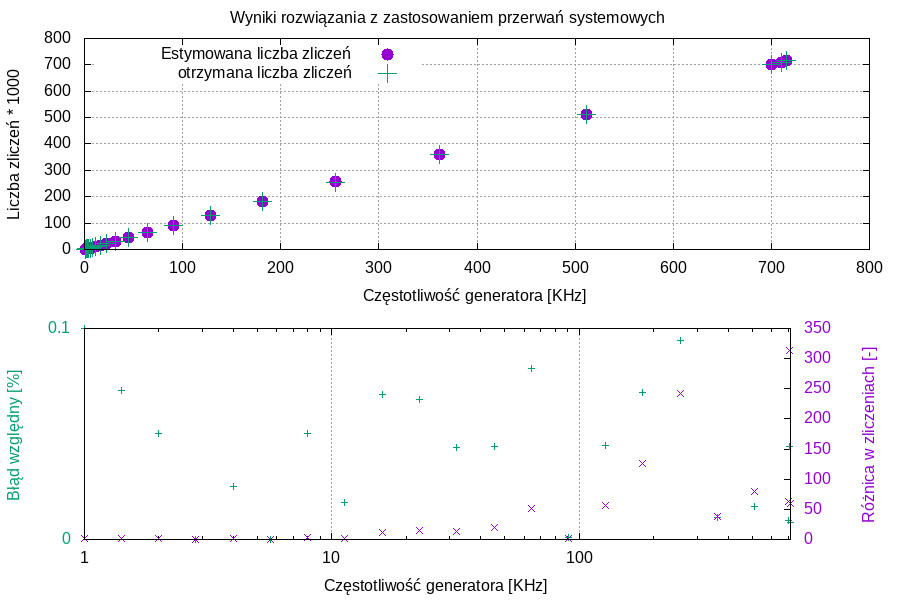
\includegraphics[width=\textwidth]{rts.jpg}
        \caption{Wyniki testów z wykorzystaniem przerwań systemowych}
        \label{rts wyniki}
\end{figure}

\begin{table}
        \centering
        \caption{Wyniki rozwiązania z zastosowaniem przerwań systemowych}
        \label{rts table}
        \begin{tabular}{|c|c|c|c|c|}  
                \hline 
                Częstotliwość [kHz] & Estymowana ilość & Otrzymana ilość & Różnica  & Błąd względny [\%]\\ 
                &  zliczeń &  zliczeń & w zliczeniach & \\ \hline
                1 & 1000 & 1001 & 1 & 0.1000\\ \hline 
                1.414 & 1414 & 1415 & 1 & 0.0707\\ \hline 
                2 & 2000 & 2001 & 1 & 0.0500\\ \hline 
                2.82 & 2820 & 2820 & 0 & 0.0000\\ \hline 
                4 & 4000 & 3999 & 1 & 0.0250\\ \hline 
                5.65 & 5650 & 5650 & 0 & 0.0000\\ \hline 
                8 & 8000 & 7996 & 4 & 0.0500\\ \hline 
                11.3 & 11300 & 11298 & 2 & 0.0177\\ \hline 
                16 & 16000 & 15989 & 11 & 0.0688\\ \hline 
                22.62 & 22620 & 22605 & 15 & 0.0663\\ \hline 
                32 & 32000 & 31986 & 14 & 0.0438\\ \hline 
                45.25 & 45250 & 45230 & 20 & 0.0442\\ \hline 
                64 & 64000 & 63948 & 52 & 0.0813\\ \hline 
                90.5 & 90500 & 90499 & 1 & 0.0011\\ \hline 
                128 & 128000 & 127943 & 57 & 0.0445\\ \hline 
                181 & 181000 & 180874 & 126 & 0.0696\\ \hline 
                256 & 256000 & 255758 & 242 & 0.0945\\ \hline 
                362 & 362000 & 361962 & 38 & 0.0105\\ \hline 
                512 & 512000 & 511920 & 80 & 0.0156\\ \hline 
                700 & 700000 & 699937 & 63 & 0.0090\\ \hline 
                710 & 710000 & 709686 & 314 & 0.0442\\ \hline 
                715 & 715000 & 714941 & 59 & 0.0083\\ \hline
        \end{tabular}
\end{table}

Wyniki pokazują dokładność mieszczącą się w  1\textperthousand, 
jednak błąd w otrzymanym wyniku zależy od częstotliwości generowanych zliczeń.
Może to być spowodowane interferencją przerwania powodującego zliczenie z innymi przerwaniami wymaganymi do działania mikrokontrolera.

Po osiągnięciu częstotliwości granicznej > 0.715 [MHz] program mikrokontrolera przestaje wysyłać dane na komputer zewnętrzny.
Jest to spowodowane tym że zaraz po wyjściu z obsługi przerwania systemowego program natychmiast zaczyna obsługę następnego przerwania. 
Liczba graniczna pozwala przybliżyć czas konieczny na wykonanie jednego przerwania na podstawie przekształcenia wzoru \ref{Cykli w sec}. 
$$ t_p = \frac{1}{f_p} = \sim 1.3986 [\mu s] $$
$$ N_c = \frac{t_p}{t_c} =  \frac{1.3986 \mu s}{11.9 ns} =\sim 118$$
gdzie: \\
        \indent $t_p$ -  czas potrzebny na obsługą przerwania\\
        \indent $t_c$ -  czas jednego cyklu procesora (dział \ref{dzial arduino} ) \\
        \indent $f_p$ -  częstotliwość graniczna przerwań \\
        \indent $N_c$ -  ilość cykli koniecznych na pojedyncze przerwanie \\

Liczba cykli na przerwanie jest mniejsza niż ta szacowana w dziale \ref{dzial arduino} (355 + 128)\cite{ard_opt_git}, wynika to z faktu że poprzednia estymacja była wykonana dla najgorszego przypadku dla nieoptymalizowanego kodu.
Mimo lepszych osiągów niż te szacowane wynik ten nadal odbiega od optymalnego czasu wywołania przerwania (12 + 10) \cite{interupt latency} i wciąż jest znacznie poniżej wymagań projektu. 

Dodatkowe testy potwierdziły że wraz z zwiększeniem ilości badanych kanałów częstotliwość graniczna zmniejsza się jak $\frac{1}{n}$ gdy $n$ to ilość badanych kanałów. 

